\documentclass[11pt,a4paper]{article}
\usepackage[utf8]{inputenc}
\usepackage{amsmath}
\usepackage{amsfonts}
\usepackage{amssymb}
\usepackage{graphicx}
\usepackage{hyperref}
\author{Ben Augarten, Richard Hwang, Max Johnson}
\title{CS 189: HW5 Report}
\begin{document}
\maketitle
\section{Features Implemented}
\begin{itemize}
\item Decision Trees
\begin{itemize}
\item Impurity Function: Entropy
\item Impurity Function: Gina
\item Impurity Function: Misclassification
\item Stopping Criteria: Number of Points
\item Stopping Criteria: Impurity Reduction
\end{itemize}
\item Random Forest
\begin{itemize}
\item Random selection of features
\item Random selection from K best split points
\end{itemize}
\item Boosted Trees (AdaBoost)
\end{itemize}
\section{Results}
\subsection{Decision Trees}
We implemented Decision Trees with 2 different stopping criteria: Stopping based on the number of points, and stopping based on the reduction of impurity. We also implemented three different impurity functions; Entropy, Gina Impurity, and Misclassification.

\subsubsection{Stopping Criteria}
Entropy, fully grown: 0.0788\\
Entropy, with leaves of at least 26 nodes: 0.0755\\
Entropy, error vs n nodes:\\
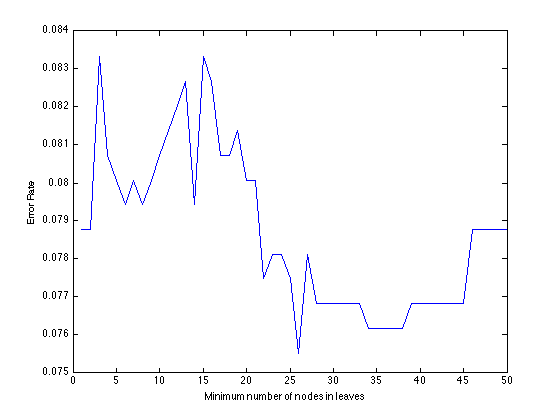
\includegraphics[width=\textwidth]{decision_tree_entropy_error_vs_n_nodes.png}
Entropy, fully grown: 0.0788\\
Entropy, with an impurity reduction cutoff of 0.6: 0.0781
Entropy, error vs n nodes:\\
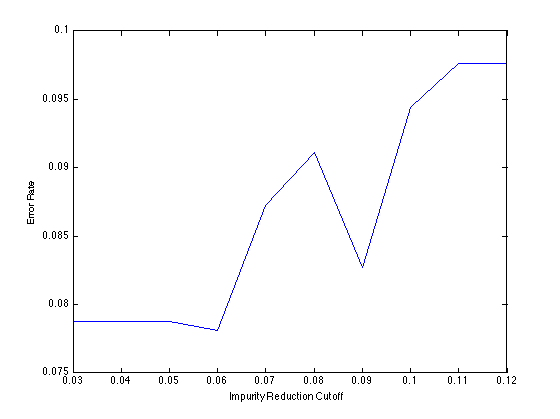
\includegraphics[width=\textwidth]{decision_tree_entropy_error_vs_imp_red.png}

\subsubsection{Impurity Functions}
Variance, fully grown: 0.0872 \\
Variance, with leaves of at least 7 nodes: 0.0846 \\
Variance, error vs n nodes:\\
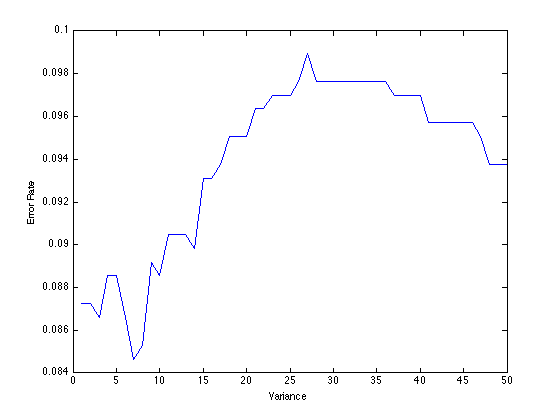
\includegraphics[width=\textwidth]{decision_tree_variance_error_vs_n_nodes.png}
Misclassification, fully grown: 0.0840\\
Misclassification, with leaves of at least 6-11 nodes: 0.0814 \\
Misclassification, error vs n nodes:\\
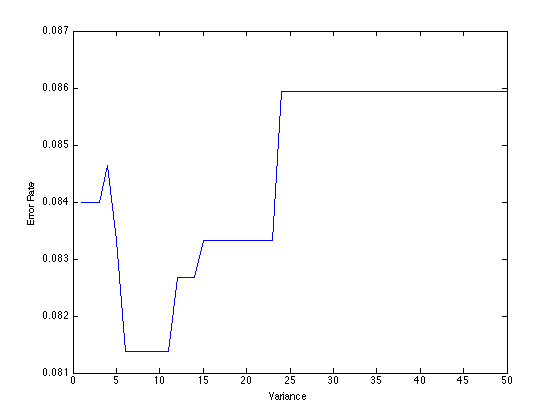
\includegraphics[width=\textwidth]{decision_tree_misclassification_error_vs_n_nodes.png}

\subsection{Random Forests}
\subsubsection{Random feature selection}
Achieved an error rate of 0.0456 with a forest of 150 nodes selecting splits from 5 random features.

\subsubsection{Random selection from top-k split points}
Achieved an error rate of 0.0612 with a forest of 200 trees, selecting from the top 200 nodes.

\subsection{Boosted Trees}
We implemented the AdaBoost algorithm by boosting weak decsion trees of depth 2. We found this worked better than stumps, as too many of the stumps were identical. \\
With 750 trees, we achieved an error rate of 0.0964. \\
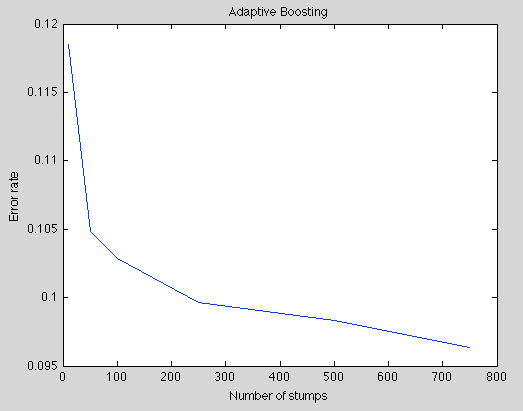
\includegraphics[width=\textwidth]{adaboost.png}

\section{Summary}
We achieved the best result using Random Forests with random feature selection. The best error rate we achieved was 4.6\%.

\section{References}
\begin{itemize}
\item Included Materials
\item \url{http://www.stat.berkeley.edu/~breiman/RandomForests/cc_home.htm}
\item \url{http://en.wikipedia.org/wiki/Random_forest}
\end{itemize}

\end{document}